
%(BEGIN_QUESTION)
% Copyright 2010, Tony R. Kuphaldt, released under the Creative Commons Attribution License (v 1.0)
% This means you may do almost anything with this work of mine, so long as you give me proper credit

An operator summons you to investigate a strange control problem she's been having on a liquid flow control loop.  This trend shows the behavior of the control loop following a major change in setpoint:

$$\includegraphics[width=15.5cm]{i01869x01.eps}$$

Instead of quickly rising to meet the new (higher) setpoint, the PV remains unchanged until it suddenly steps up (twice!) toward the new setpoint.  The controller output, meanwhile, continues to drive upward.

\vskip 10pt

Given what you see here, identify one or more likely causes of this strange behavior.  What other diagnostic tests might you do next, and where would you concentrate your search for problems in the system?

\vskip 20pt \vbox{\hrule \hbox{\strut \vrule{} {\bf Suggestions for Socratic discussion} \vrule} \hrule}

\begin{itemize}
\item{} Follow along the trend from left to right (progressing forward in time), narrating what the trend says about the process variable, the setpoint, and the controller output over time.  It is a good problem-solving technique to do this {\it first} before arriving at any conclusions as to what is wrong with the loop.
\item{} Do you think this controller is {\it proportional-only}, {\it integral-only}, or {\it P+I}?  How can you tell?
\item{} What would the trend look like if this controller implemented some {\it other} kind of action?
\item{} An immediate response of some technicians is to begin changing the controller's tuning constants (gain, reset period, etc.) when they see poor control response on a trend.  Do you think this would be a wise decision in this particular case?  Why or why not?
\end{itemize}

\underbar{file i01869}
%(END_QUESTION)





%(BEGIN_ANSWER)

The control valve is most likely sticky.

%(END_ANSWER)





%(BEGIN_NOTES)

By a ``sticky'' valve, I mean the valve exhibits excessive friction in its travel.  For a pneumatically actuated control valve, this leads to a behavior often called a {\it slip-stick} cycle.

%INDEX% Process troubleshooting: diagnosing problem via trend recording

%(END_NOTES)


